	\begin{figure}[!h]
		\centering
 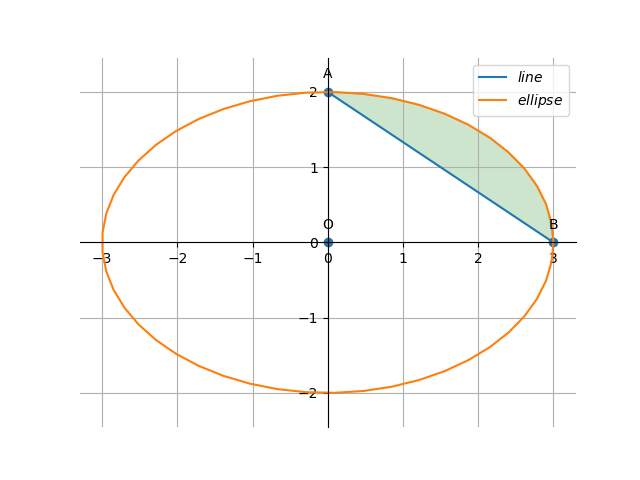
\includegraphics[width=\columnwidth]{chapters/12/8/3/8/figs/conic_fig.png}
		\caption{}
		\label{fig:12/8/3/8}
  	\end{figure}
The given ellipse can be expressed as conics with parameters
\begin{align}
\vec{V}=\myvec{
b^2 & 0\\
0 & a^2
},
\vec{u}=0,
f=-(a^2b^2).
\end{align} 
The line parameters are
\begin{align}
\vec{h} &= \myvec{
a\\
0
},
\vec{m} = \myvec{\frac{1}{b} \\ -\frac{1}{a}}.
\end{align}
Substituting the given parameters in \eqref{eq:tangent_roots},
\begin{align}
    \mu=0,-6
\end{align}
yielding the points of intersection
\begin{align}
    \vec{A}=\myvec{
a\\
0
    },
    \vec{B}=\myvec{
0\\
b
    }.
\end{align}
From 
		\figref{fig:12/8/3/8},
the desired area is
\begin{multline}
\int_{0}^{a}\frac{b}{a}\sqrt{a^2-x^2} \,dx 
-\int_{0}^{a} \frac{b}{a}(a-x) \,dx
\\
	= \frac{ab}{2}\brak{\frac{\pi}{2}-1}
	= 3\brak{\frac{\pi}{2}-1}
\end{multline}
upon substituting $a=3, b=2$.
